\documentclass{beamer}
%
% Choose how your presentation looks.
%
% For more themes, color themes and font themes, see:
% http://deic.uab.es/~iblanes/beamer_gallery/index_by_theme.html
%
\mode<presentation>
{
  \usetheme{Boadilla}      % or try Darmstadt, Madrid, Warsaw, ...
  \usecolortheme{beaver} % or try albatross, beaver, crane, ...
  \usefonttheme{default}  % or try serif, structurebold, ...
  \setbeamertemplate{navigation symbols}{}
  \setbeamertemplate{caption}[numbered]
  
} 

\usepackage{xcolor,colortbl}
\usepackage[english]{babel}
\usepackage[utf8x]{inputenc}
\usepackage{courier}
\usepackage{dsfont}
\usepackage{verbatim} 
\usepackage{enumerate}
\usepackage{tikz}
\usepackage{multirow}
\usepackage{venndiagram}
\usepackage{epigraph} 
%\usepackage{xcolor}
\usepackage{makecell}

%\usepackage{enumitem}

\usepackage{hyperref}
\hypersetup{
    colorlinks=true,
    linkcolor=blue,
    filecolor=magenta,      
    urlcolor=cyan,
}

% R stuff!
\usepackage{listings}
\definecolor{codegreen}{rgb}{0,0.6,0}
\definecolor{codegray}{rgb}{0.5,0.5,0.5}
\definecolor{codepurple}{rgb}{0.58,0,0.82}
\definecolor{backcolour}{rgb}{0.95,0.95,0.92}

\lstdefinestyle{mystyle}{
    backgroundcolor=\color{backcolour},    
    commentstyle=\color{codegreen},
    keywordstyle=\color{black},
    numberstyle=\tiny\color{codegray},
    stringstyle=\color{codepurple},
    basicstyle=\ttfamily\footnotesize,
    breakatwhitespace=false,         
    breaklines=true,                 
    captionpos=b,                    
    keepspaces=true,                 
    numbers=left,                    
    numbersep=5pt,                  
    showspaces=false,                
    showstringspaces=false,
    showtabs=false,                  
    tabsize=2
}

\lstset{style=mystyle}


\setbeamertemplate{enumerate items}[default]
\setbeamertemplate{itemize item}[triangle]

%\setitemize{label=\usebeamerfont*{itemize item}%
%  \usebeamercolor[fg]{itemize item}
%  \usebeamertemplate{itemize item}}



\title[Introduction to Statistics]{Bootstrapping}
\subtitle{Alternative to Normal and t-distributions}
\author{Grinnell College}
\date{}

\graphicspath{{img/}}

\begin{document}

\begin{frame}
  \titlepage
\end{frame}

\begin{frame}{Review}
We have seen how to make Confidence Intervals to estimate
\begin{itemize}
    \item population mean ($\mu$)
    \item difference in pop. means ($\mu_1 - \mu_2$)
    \item population proportion (p)
    \item difference in pop. proportions ($p_1 - p_2$)
\end{itemize} \vspace{6mm}

Methods
\begin{itemize}
    \item Normal distribution (p, $p_1 - p_2$)
    \item t-distribution ($\mu$, $\mu_1 - \mu_2$)
\end{itemize}
\end{frame}

\begin{frame}{Review}
\textbf{Sampling distribution}
\begin{itemize}
    \item Distribution of statistics from many samples
    \item Shows us variability in the statistics
\end{itemize} \vspace{6mm}

CIs so far have been based on \textbf{CLT}
\begin{itemize}
    \item For a large enough sample size, the sampling distribution for a sample mean (or proportion) looks like a Normal distribution
\end{itemize}
\end{frame}

\begin{frame}{Outline}
\textbf{Motivation} for today: What do we do when we want to estimate things other than means and proportions?
\begin{itemize}
    \item CI for median, IQR, standard deviation?
    \item We can't use Normal/t because CLT doesn't work for these
\end{itemize} \vspace{12mm}

We will see an alternative approach to estimate these with a CI.
\end{frame}

\begin{frame}{Repeated Samples}
\footnotesize

Confidence intervals we constructed had the form:
\begin{align*}
\text{Point Estimate} \pm \text{Margin of Error}
\end{align*}
\vspace{-6mm}
\begin{itemize}
\item Relied on assumptions about populations and CLT
\item Examined what might happen if we could repeat sampling ad infinitum
\end{itemize}
\end{frame}

\begin{frame}{Review -- Sampling Distribution}
\begin{center}
    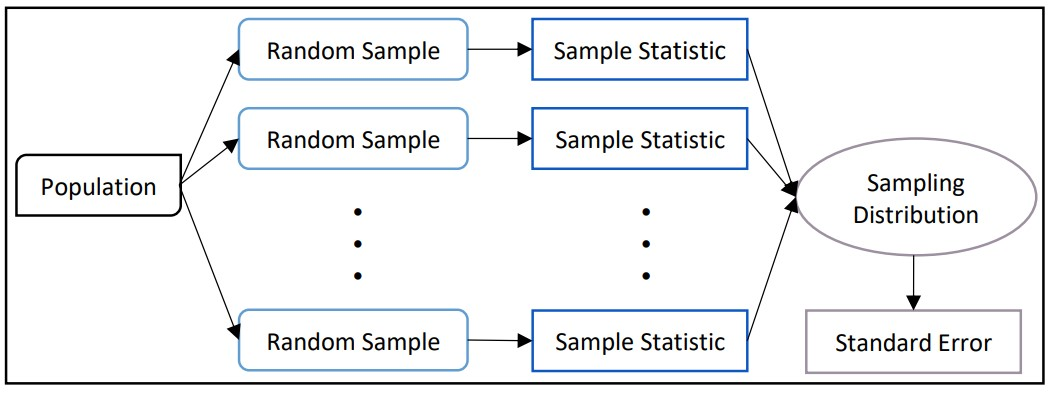
\includegraphics[scale=.6]{img/sampling_distr_method.jpg}
\end{center}
How to construct?
\begin{enumerate}
    \item Start with population.
    \item Take a sample and compute the statistic of choice
    \item Take another sample and compute the statistics
    \item Continue to take more samples and compute statistic each time
    \item Plot all of the statistics in a histogram or dotplot
\end{enumerate}
\end{frame}

\begin{frame}{Issues?}
There are, naturally, some limitations:
\begin{itemize}
\item We are limited to collecting a single sample
\item So... Can't make a sampling distribution in reality
\end{itemize}
\end{frame}

\begin{frame}{Bootstrapping}
Our solution is something called \textbf{"Bootstrapping"}
\vspace{8mm}

\textbf{Bootstrapping:} 

Instead of taking a lot of samples from the population over and over...
\begin{itemize}
    \item Bootstrapping simulates this process
    \item Create many "new samples" using the original sample we collect
\end{itemize} \vspace{8mm}

\textbf{Logic:}
\begin{enumerate}
    \item If sample is randomly selected $\rightarrow$ representative
    \item Make many copies of the sample $\rightarrow$ approximation of the population
    \item Take samples from "new population" $\rightarrow$ approximates sampling dist.
    \item Now we can make CI's
\end{enumerate}
\end{frame}

\begin{frame}{Bootstrapping}
\textbf{Method:}
\begin{enumerate}
    \item Random sample is representative of population
    \item Use the sample as a proxy for the population
    \item Draw new samples (with replacement) from the original sample
    \item Sample size of new samples must match the original
\end{enumerate}

\begin{center}
    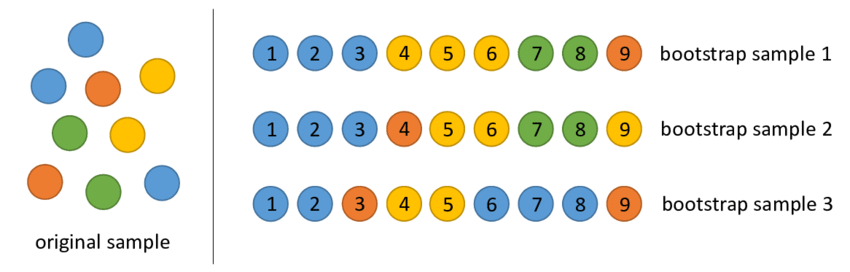
\includegraphics[scale=.4]{img/bootstrap_pic.png}
\end{center}
\end{frame}

\begin{frame}{Bootstrapping}
\textbf{Method:}
\begin{enumerate}
    \item Random sample is representative of population
    \item Use the sample as a proxy for the population
    \item Draw new samples (with replacement) from the original sample
    \item Sample size of new samples must match the original
\end{enumerate}
\begin{center}
    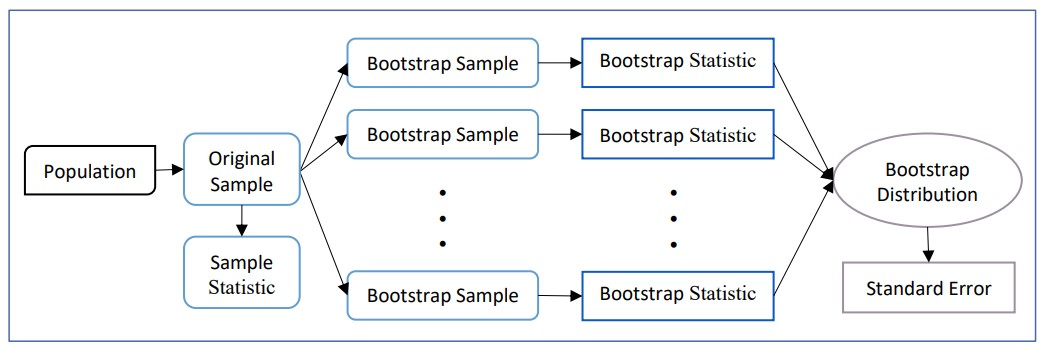
\includegraphics[scale=.6]{img/bootstrap_process.jpg}
\end{center}
\end{frame}

\begin{frame}{Comparison}
Sampling Distribution: new samples from population
\begin{center}
    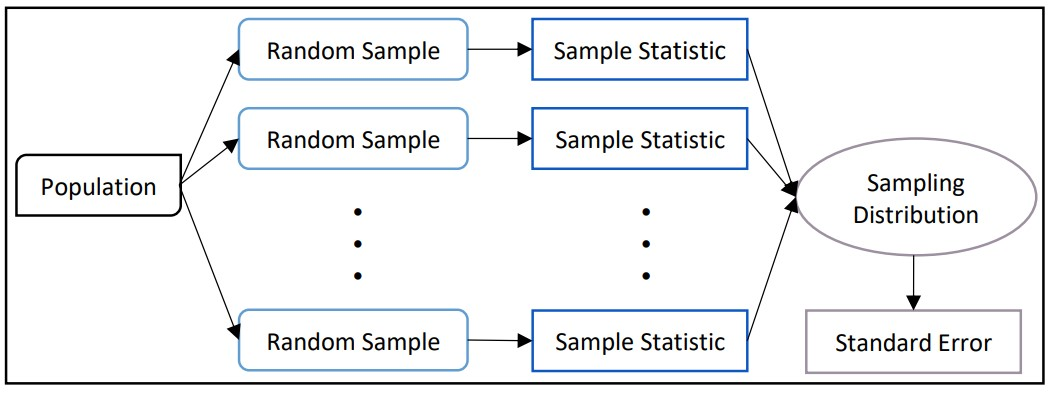
\includegraphics[scale=.49]{img/sampling_distr_method.jpg}
\end{center}

Bootstrap Distribution: new samples from the original sample
\begin{center}
    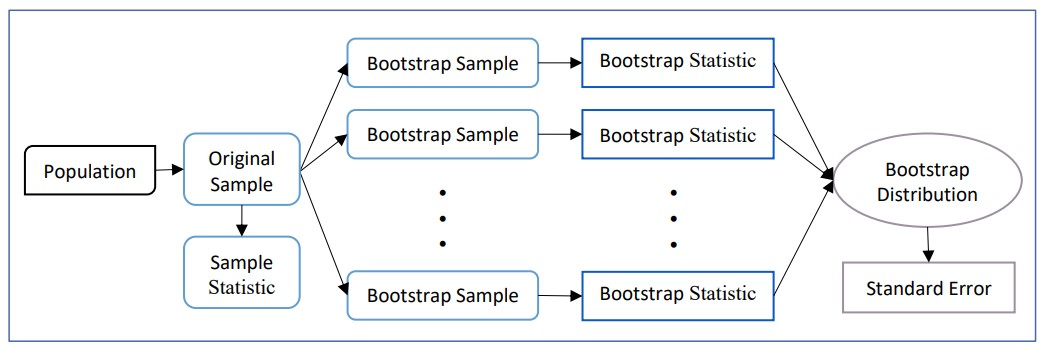
\includegraphics[scale=.5]{img/bootstrap_process.jpg}
\end{center}
\end{frame}

\begin{frame}{Rainfall Example}
We have data collected on the amount of precipitation on 121 rainy days in Grinnell from 2014-2024 (courtesy of Professor Nolte) \vspace{2mm}

\begin{center}
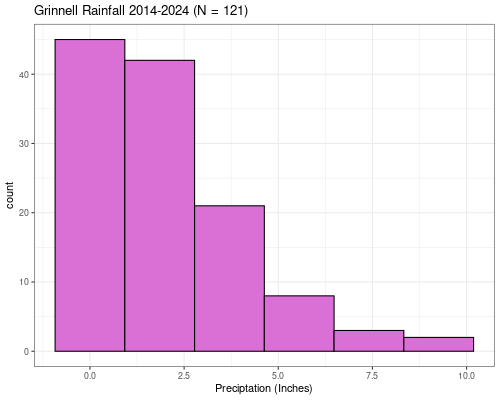
\includegraphics[scale=0.48]{grin_rain.png}
\end{center}
\end{frame}

\begin{frame}{Rainfall Example}
Let's say we took a random sample of 30 rainy days...
\begin{columns}

  \begin{column}{0.45\textwidth}
\begin{center}
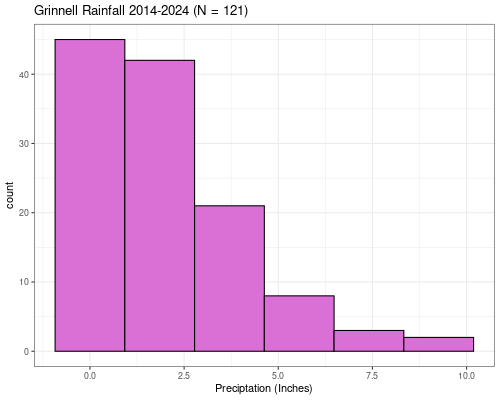
\includegraphics[scale=0.32]{grin_rain.png}
\end{center}
  \end{column}
  \begin{column}{0.45\textwidth}
\begin{center}
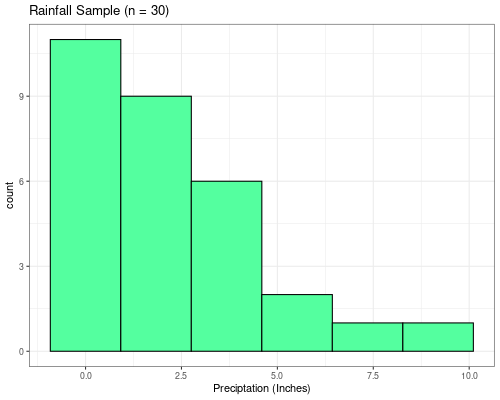
\includegraphics[scale=0.32]{grin_rain_samp.png}
\end{center}
  \end{column}

\end{columns}
\begin{itemize}
    \item Random sample $\rightarrow$ representative
    \item Same shape, very similar center and spread
\end{itemize}
\end{frame}

\begin{frame}{Rainfall Example}
Start the bootstrap process.
\begin{itemize}
    \item Make some bootstrap samples of size 30
    \item Do they \textit{kind of} look the same? Yeah!
\end{itemize}
\begin{columns}

  \begin{column}{0.45\textwidth}
\begin{center}
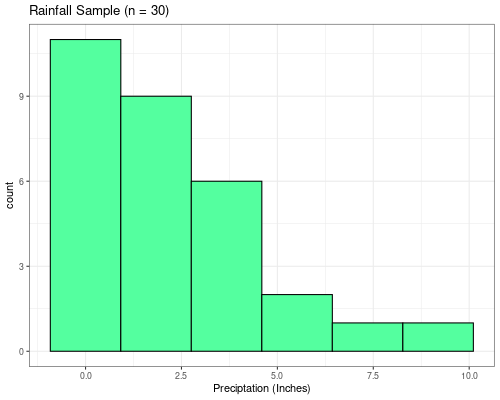
\includegraphics[scale=0.32]{grin_rain_samp.png}
\end{center}
  \end{column}
  \begin{column}{0.45\textwidth}
\begin{center}
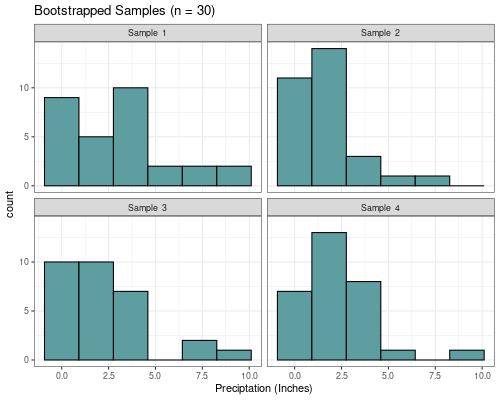
\includegraphics[scale=0.32]{grin_rain_boot.png}
\end{center}
  \end{column}

\end{columns}
\end{frame}

\begin{frame}{Rainfall Example}
More bootstrap samples...
\begin{center}
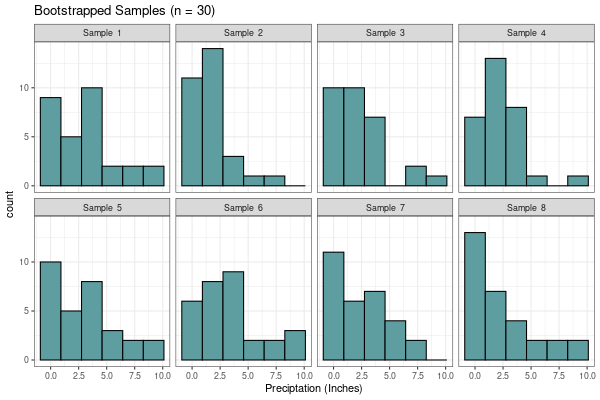
\includegraphics[scale=0.5]{grin_rain_boot2.png}
\end{center}
\end{frame}

\begin{frame}{Rainfall Example}
Compute the mean of each bootstrap sample...
\begin{center}
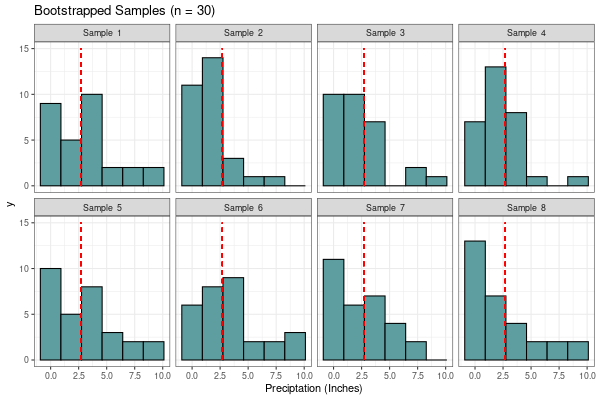
\includegraphics[scale=0.5]{grin_rain_boot3.png}
\end{center}
\end{frame}

\begin{frame}{Rainfall Example}
Graph the means from the bootstrap samples $\rightarrow$ \textbf{Bootstrap Distribution}
\begin{center}
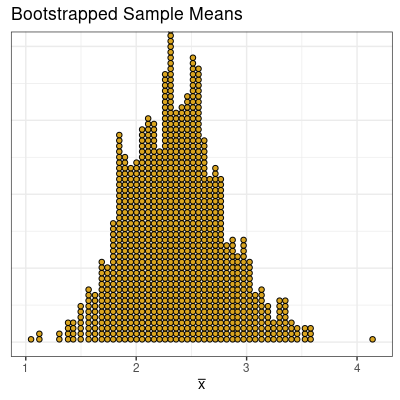
\includegraphics[scale=0.65]{img/mean_bootstrap2.png}
\end{center}
\end{frame}

\begin{frame}{Back to CI's}
We can use the bootstrap distribution to make CI's without needing to go back to Normal or t-distribution stuff
\end{frame}

\begin{frame}{Percentiles}
Remember percentiles?
\begin{itemize}
    \item A value where some \% of the distribution is below that value
    \item ex) median (50th percentile), Q1, Q3
\end{itemize} \vspace{8mm}

\textbf{Question:} What \% of \textit{any} distribution is between the 97.5 percentile and the 2.5 percentile?
\end{frame}

\begin{frame}{Bootstrap Percentiles}
\begin{center}
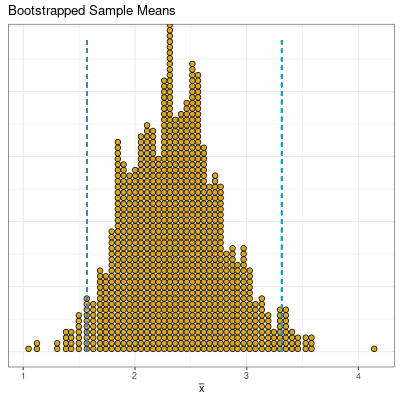
\includegraphics[scale=0.42]{img/mean_bootstrap_perc.png}
\end{center}
95\% of bootstrap sample means are between the 2.5 percentile and the 97.5 percentile
\begin{itemize}
    \item This constitutes a 95\% confidence interval!
\end{itemize}
\end{frame}

\begin{frame}{More on Bootstrapping}
\textbf{Other \% CI's?} Use different percentiles to make the CI
\begin{itemize}
    \item 80\% CI $\rightarrow$ 10 and 90 percentiles
    \item 90\% CI $\rightarrow$ 5 and 95 percentiles
    \item 95\% CI $\rightarrow$ 2.5 and 97.5 percentiles
    \item 99\% CI $\rightarrow$ 0.5 and 99.5 percentiles
\end{itemize}
\end{frame}

\begin{frame}{More on Bootstrapping}
\textbf{Benefits:}
\begin{itemize}
    \item Can use bootstrapping for things other than means or proportions
    \item Don't need to rely on Normal / t-distributions
    \begin{itemize}
        \item use when Normal / t-distribution conditions aren't met
    \end{itemize}
\end{itemize} \vspace{8mm}

\textbf{Downsides:}
\begin{itemize}
    \item Need access to computer to simulate bootstrap process
    \item bootstrap CIs are often wider than Normal/t-distribution intervals
\end{itemize}

\end{frame}

%%%%%%%%%%%%%%%%

%\begin{frame}
%\begin{columns}
%
%  \begin{column}{0.45\textwidth}
%%
%  \end{column}
%  \begin{column}{0.45\textwidth}
%%
%  \end{column}
%
%\end{columns}
%\end{frame}


\end{document}